\chapter{实验研究}

本章主要通过实验来验证所选用硬件组成自动分拣系统的可用性、稳定性和准确定,以及所选用目标检测算法的优越性。然后通过实验
验证深度学习云平台的可用性与稳定性。第一部分将针对自动分拣系统的分拣延时和分拣准确率进行实验,对YOLOv3和YOLOv3-tiny在
自动分拣系统中的延时进行对比与选择。然后对应用YOLOv3-tiny的自动分拣系统的分拣准确率进行实验。第二部分针对深度学习云平台的
Web前端和服务器后端进行了性能稳定性测试。

\section{机械臂分拣系统性能实验}

本节将所设计的基于深度学习的自动分拣系统进行实验,包括图像处理模块的延时实验和分拣准确率实验。其中,延时实验主要是将YOLOv3和YOLOv3-tiny
部署在自动分拣系统后的延时进行对比,从而验证选择YOLOv3-tiny模型配置的优越性。分拣准确率实验又包括
分拣分类准确率实验和抓取成功率实验。前者主要衡量图像处理模块将工件进行准确分类的能力,后者主要衡量图像处理模块识别工件边框
的能力。

本实验中,硬件平台如表\ref{table:exper:hardware}所示。

{
    \begin{table}[htb] 
        \zihao{5}
        \caption{实验各硬件平台配置表}
        \label{table:exper:hardware}
        \centering
        \begin{tabular}[t]{c|c|c|c|c|c}
            \hline
            工件 & 摄像头 & 图像处理平台 & 机械臂 & 显示器 & 服务器  \\
            \hline
            3D打印工件 & 罗技C270 & Jetson TX2 & DOBOT & AOC I2490VXH & DELL T630 \\
            \hline 
        \end{tabular} 
    \end{table}
}

上表所示配置即第二章中所介绍的自动分拣系统的硬件选型配置。实验环境下为自动分拣系统的Jetson TX2配备了显示器,
主要目的为观测目标检测的效果实况,以及记录当前图像处理的FPS。此外,实验环境和实际使用中,Jetson TX2开启最大功耗模式。

软件环境如表\ref{table:exper:software}所示。

{
    \begin{table}[htb] 
        \zihao{5}
        \caption{实验软件环境配置表}
        \label{table:exper:software}
        \centering
        \begin{tabular}[t]{c|c|c|c|c|c}
            \hline
            操作系统 & 模块通信 & G-Code支持 & 算法部署 & 编译工具 & 脚本环境  \\
            \hline
            Linux tegra-ubuntu & USB/ROS/串口 & Marlin固件 & darknet\_ros & catkin\_make & Python/Shell \\
            \hline 
        \end{tabular} 
    \end{table}
}

分拣延时的实验数据通过修改自动分拣系统图像处理模块代码直接将数据保存到本地得到;分拣准确率的实验数据通过人工放置工件和人工观察记录得到。


\subsection{自动分拣系统图像处理模块算法性能试验}

本文第三章第三节中已对YOLOv3和YOLOv3-tiny的性能进行了比较,该比较基于服务器环境,非部署环境。因此本小节将对部署后两者的性能进行对比试验,以
验证针对本任务YOLOv3-tiny配置的优越性。

使用darknet\_ros分别将YOLOv3和YOLOv3-tiny配置的模型部署到自动分拣系统的图像处理模块进行延时实验。实验比较参数为FPS(Frame per Second),即图像处理模块预测图片后显示到显示器
上的帧率。该参数可以反映出图像处理模块进行图像预测的能力,即每秒能够处理的图片数量。实验采集了两个模型部署后处理图片的50个瞬时FPS数据,
数据采集如表\ref{table:delay:data}所示。

{
    \begin{table}[htb] 
        \zihao{5}
        \caption{延时实验数据采集表}
        \label{table:delay:data}
        \centering
        \begin{tabular}[t]{c|c|c|c|c|c|c|c|c|c|c}
            \hline
            \diagbox{配置}{FPS}{编号} & 1 & 2 & 3 & 4 & 5 & 6 & 7 & 8 & 9 & 10 \\
            \hline
            YOLOv3 & 1.51 & 1.48 & 1.49 & 1.53 & 1.56 & 1.50 & 1.54 & 1.55 & 1.40 & 1.48\\
            %%\hline 
            YOLOv3-tiny & 14.92 & 15.20 & 15.49 & 14.65 & 14.90 & 14.78 & 14.56 & 15.50 & 15.18 & 15.04\\
            \hline
            & 11 & 12 & 13 & 14 & 15 & 16 & 17 & 18 & 19 & 20 \\
            \hline
            YOLOv3 & 1.49 & 1.54 & 1.52 & 1.54 & 1.51 & 1.40 & 1.44 & 1.49 & 1.47 & 1.52\\
            %%\hline 
            YOLOv3-tiny & 15.41 & 15.10 & 15.19 & 15.65 & 14.98 & 15.12 & 15.34 & 14.90 & 14.88 & 14.72\\
            \hline
            & 21 & 22 & 23 & 24 & 25 & 26 & 27 & 28 & 29 & 30 \\
            \hline
            YOLOv3 & 1.38 & 1.46 & 1.42 & 1.52 & 1.54 & 1.44 & 1.53 & 1.45 & 1.50 & 1.52\\
            %%\hline 
            YOLOv3-tiny & 15.01 & 15.22 & 15.05 & 15.43 & 14.87 & 15.23 & 15.04 & 14.81 & 14.78 & 14.92\\
            \hline
            & 31 & 32 & 33 & 34 & 35 & 36 & 37 & 38 & 39 & 40 \\
            \hline
            YOLOv3 & 1.49 & 1.50 & 1.56 & 1.42 & 1.50 & 1.41 & 1.43 & 1.53 & 1.55 & 1.51\\
            %%\hline 
            YOLOv3-tiny & 14.91 & 14.92 & 15.32 & 15.51 & 14.85 & 14.66 & 14.94 & 15.20 & 14.68 & 15.15\\
            \hline
            & 41 & 42 & 43 & 44 & 45 & 46 & 47 & 48 & 49 & 50 \\
            \hline
            YOLOv3 & 1.53 & 1.52 & 1.54 & 1.52 & 1.48 & 1.51 & 1.50 & 1.53 & 1.49 & 1.50\\
            %%\hline 
            YOLOv3-tiny & 14.95 & 15.04 & 15.22 & 15.21 & 15.15 & 14.92 & 15.01 & 14.88 & 15.02 & 15.27\\
            \hline
        \end{tabular} 
    \end{table}
}

两个模型瞬时FPS曲线图及平均FPS对比如图\ref{fig:FPS}所示。


\begin{figure}[h]
    \centering
    \subfigure[瞬时FPS曲线图]{
        \label{fig:FPS:moment}
        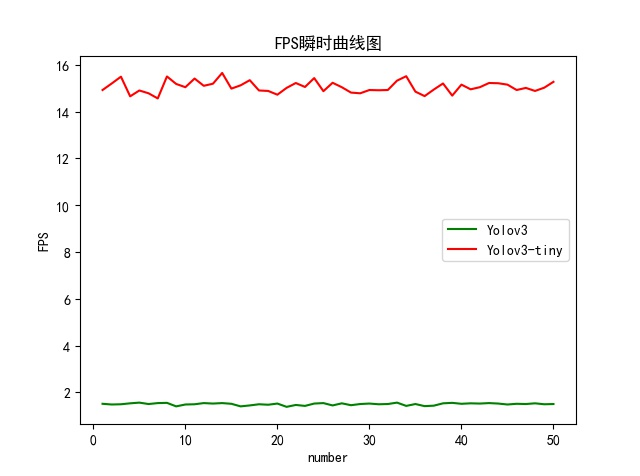
\includegraphics[width=0.46\columnwidth]{pic/chap5/FPS_plot.jpeg}
    }
    \subfigure[平均FPS柱状图]{
        \label{fig:FPS:average}
        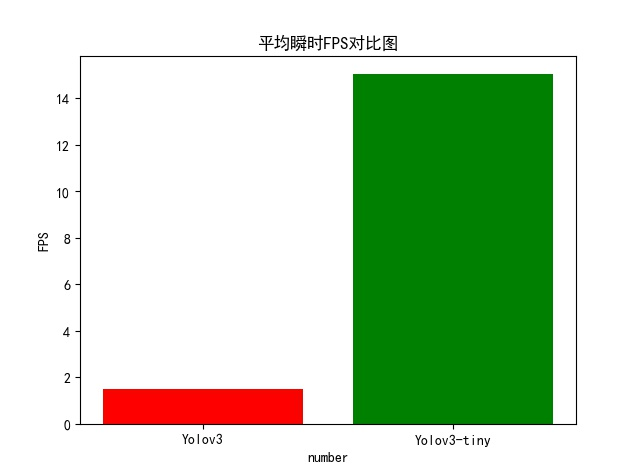
\includegraphics[width=0.46\columnwidth]{pic/chap5/average_FPS_plot.jpeg}
    }
    \caption{YOLOv3和YOLOv3-tiny部署后的FPS对比}
    \label{fig:FPS}
\end{figure}

由数据表及上图可知,YOLOv3部署后的FPS值稳定在1.50附近,平均值为1.4948;YOLOv3-tiny部署后的FPS值稳定在15.0附近,平均值为15.0536。
YOLOv3-tiny的FPS约为YOLOv3的10倍,即YOLOv3-tiny在一秒内能够处理的图片数量十倍于YOLOv3。

此外,实验还比较了两者在实验环境的新数据下的分类准确率。比较参数为51次实验情况下,每个工件的分类准确率。实验数据采集如下表:

{
    \begin{table}[htb] 
        \zihao{5}
        \caption{YOLOv3分类准确率实验数据采集表}
        \label{table:classification:YOLOv3_data}
        \centering
        \begin{tabular}[t]{c|c|c|c|c|c|c|c|c|c|c|c|c|c|c|c|c|c}
            \hline
            \diagbox{模型配置}{实验编号} & 1 & 2 & 3 & 4 & 5 & 6 & 7 & 8 & 9 & 10 & 11 & 12 & 13 & 14 & 15 & 16 & 17\\
            \hline
            dabai是否正确分类 & 1 & 1 & 0 & 1 & 1 & 1 & 1 & 1 & 1 & 1 & 1 & 1 & 1 & 1 & 1 & 1 & 1\\
            fo是否正确分类 & 1 & 1 & 1 & 1 & 1 & 1 & 1 & 1 & 1 & 1 & 1 & 1 & 1 & 1 & 1 & 0 & 1\\
            \hline
            & 18 & 19 & 20 & 21 & 22 & 23 & 24 & 25 & 26 & 27 & 28 & 29 & 30 & 31 & 32 & 33 & 34 \\
            \hline
            dabai是否正确分类 & 1 & 1 & 1 & 1 & 1 & 1 & 1 & 1 & 1 & 0 & 1 & 1 & 1 & 1 & 1 & 1 & 1\\
            fo是否正确分类 & 1 & 1 & 1 & 1 & 1 & 1 & 1 & 1 & 1 & 1 & 1 & 1 & 1 & 1 & 1 & 1 & 1\\
            \hline
            & 35 & 36 & 37 & 38 & 39 & 40 & 41 & 42 & 43 & 44 & 45 & 46 & 47 & 48 & 49 & 50 & 51\\
            \hline
            dabai是否正确分类 & 1 & 1 & 1 & 1 & 1 & 1 & 1 & 1 & 1 & 1 & 1 & 1 & 1 & 1 & 1 & 1 & 1\\
            fo是否正确分类 & 1 & 0 & 1 & 1 & 1 & 1 & 0 & 1 & 1 & 1 & 1 & 1 & 1 & 1 & 1 & 1 & 1\\
            \hline
        \end{tabular}
    \end{table}
}

{
    \begin{table}[htb] 
        \zihao{5}
        \caption{YOLOv3-tiny分类准确率实验数据采集表}
        \label{table:classification:YOLOv3-tiny_data}
        \centering
        \begin{tabular}[t]{c|c|c|c|c|c|c|c|c|c|c|c|c|c|c|c|c|c}
            \hline
            \diagbox{模型配置}{实验编号} & 1 & 2 & 3 & 4 & 5 & 6 & 7 & 8 & 9 & 10 & 11 & 12 & 13 & 14 & 15 & 16 & 17\\
            \hline
            dabai是否正确分类 & 1 & 1 & 0 & 1 & 1 & 1 & 1 & 1 & 1 & 1 & 1 & 1 & 1 & 1 & 0 & 1 & 1\\
            fo是否正确分类 & 1 & 1 & 1 & 1 & 1 & 1 & 1 & 0 & 1 & 1 & 1 & 1 & 1 & 1 & 1 & 1 & 1\\
            \hline
            & 18 & 19 & 20 & 21 & 22 & 23 & 24 & 25 & 26 & 27 & 28 & 29 & 30 & 31 & 32 & 33 & 34 \\
            \hline
            dabai是否正确分类 & 1 & 1 & 1 & 1 & 1 & 1 & 1 & 0 & 1 & 1 & 1 & 1 & 1 & 1 & 1 & 1 & 1\\
            fo是否正确分类 & 1 & 1 & 1 & 1 & 0 & 1 & 1 & 1 & 1 & 1 & 1 & 1 & 1 & 1 & 1 & 0 & 1\\
            \hline
            & 35 & 36 & 37 & 38 & 39 & 40 & 41 & 42 & 43 & 44 & 45 & 46 & 47 & 48 & 49 & 50 & 51\\
            \hline
            dabai是否正确分类 & 1 & 1 & 1 & 1 & 1 & 1 & 1 & 1 & 1 & 1 & 1 & 1 & 1 & 1 & 0 & 1 & 1\\
            fo是否正确分类 & 1 & 1 & 1 & 1 & 1 & 1 & 1 & 1 & 1 & 1 & 1 & 1 & 1 & 1 & 1 & 1 & 1\\
            \hline
        \end{tabular}
    \end{table}
}

表中,1代表正确分类,0代表没有正确分类。分类准确率的计算方式为:
\begin{equation}
    \centering
    \mbox{分类准确率}=\mbox{正确分类样本数}/\mbox{总样本数}
    \label{acc}
\end{equation}

两种模型配置的正确分类数量和分类准确率情况对比如图\ref{fig:classification:compare}所示。

由图可知,YOLOv3的分类准确率略高于YOLOv3-tiny,但两者相差不大,而YOLOv3-tiny部署在Jetson TX2后的图像处理性能十倍于YOLOv3,因此针对本自动分拣系统,
YOLOv3-tiny的模型配置具备相当的优越性,本文最终也选定YOLOv3-tiny作为最终部署在自动分拣系统当中的目标检测算法的模型配置。

\begin{figure}[h]
    \centering
    \subfigure[YOLOv3和YOLOv3-tiny分类情况]{
        \label{fig:classification:num}
        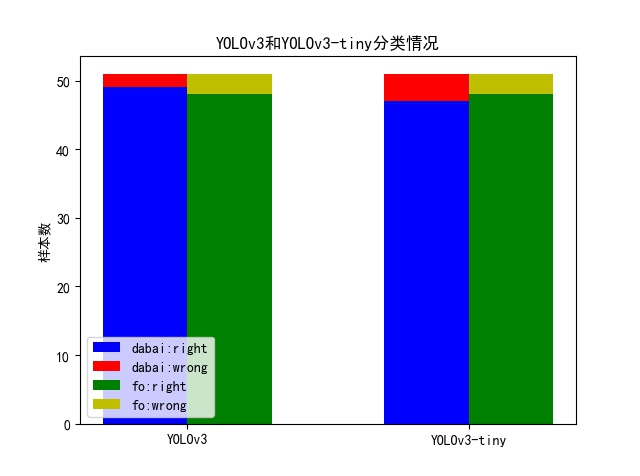
\includegraphics[width=0.46\columnwidth]{pic/chap5/classification_num.jpeg}
    }
    \subfigure[YOLOv3和YOLOv3-tiny分类准确率对比]{
        \label{fig:classification:acc}
        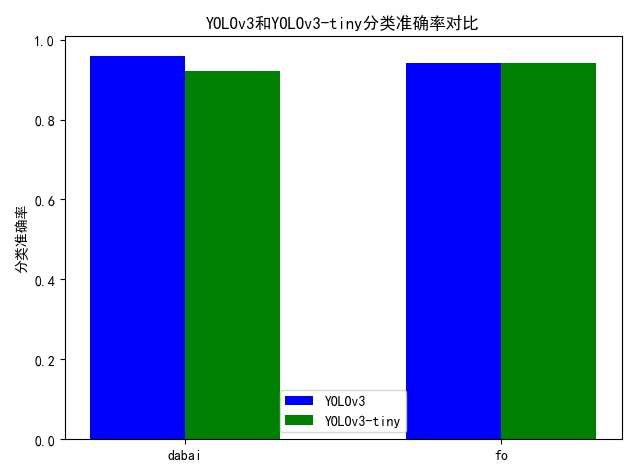
\includegraphics[width=0.46\columnwidth]{pic/chap5/classification_acc.jpeg}
    }
    \caption{YOLOv3和YOLOv3-tiny部署后的分类性能对比}
    \label{fig:classification:compare}
\end{figure}



\subsection{自动分拣系统分拣性能实验}

采用YOLOv3-tiny模型配置作为自动分拣系统图像处理模块的目标检测算法的配置进行部署,具体配置参数见表\ref{table:model:config}。
本小节将对自动分拣系统的分拣性能进行实验。分拣性能评估的是自动分拣系统能够成功抓取工件并将其正确分类的能力。因此,本实验将评估
两个实验数据:抓取成功率和分拣成功率。其中,分拣成功代表自动分拣系统将工件抓取到了正确的位置。即,抓取成功不代表分拣成功,而分拣成功代表一定抓取成功。
分拣成功率是更加严格的评估指标。抓取成功率代表自动分拣系统识别工件边框的准确能力,分拣成功率代表自动分拣系统的功能实现准确率。两者的计算方式如下:
$$\mbox{抓取成功率}=\mbox{机械臂成功抓取样本数}/\mbox{总样本数}$$
\begin{equation}
    \centering
    \mbox{分拣成功率}=\mbox{成功抓取到正确位置的样本数}/\mbox{总样本数}
    \label{fenjian}
\end{equation}

分别将两种工件dabai和fo放置在自动分拣系统的摄像头下,观测其抓取情况,记录其抓取成功和分拣成功的情况。
其中,工件dabai的数据记录表如表\ref{table:fenjian:dabai}所示;
工件fo的数据记录表如表\ref{table:fenjian:fo}所示。

{
    \begin{table}[htb] 
        \zihao{5}
        \caption{针对工件dabai的分拣性能实验数据记录表}
        \label{table:fenjian:dabai}
        \centering
        \begin{tabular}[t]{c|c|c|c|c|c|c|c|c|c|c|c|c|c|c|c|c|c}
            \hline
            \diagbox{参数}{实验编号} & 1 & 2 & 3 & 4 & 5 & 6 & 7 & 8 & 9 & 10 & 11 & 12 & 13 & 14 & 15 & 16 & 17\\
            \hline
            是否成功抓取 & 1 & 1 & 1 & 0 & 1 & 1 & 1 & 1 & 1 & 1 & 1 & 1 & 1 & 1 & 1 & 0 & 1\\
            是否正确分拣 & 1 & 1 & 1 & 0 & 1 & 1 & 1 & 1 & 1 & 1 & 1 & 1 & 1 & 1 & 0 & 0 & 1\\
            \hline
            & 18 & 19 & 20 & 21 & 22 & 23 & 24 & 25 & 26 & 27 & 28 & 29 & 30 & 31 & 32 & 33 & 34 \\
            \hline
            是否成功抓取 & 1 & 1 & 1 & 1 & 1 & 1 & 1 & 1 & 1 & 1 & 1 & 1 & 1 & 1 & 1 & 1 & 1\\
            是否正确分拣 & 1 & 1 & 1 & 1 & 1 & 1 & 1 & 1 & 1 & 1 & 1 & 1 & 1 & 1 & 1 & 1 & 1\\
            \hline
            & 35 & 36 & 37 & 38 & 39 & 40 & 41 & 42 & 43 & 44 & 45 & 46 & 47 & 48 & 49 & 50 & 51\\
            \hline
            是否成功抓取 & 1 & 1 & 1 & 1 & 1 & 1 & 1 & 1 & 1 & 1 & 1 & 1 & 1 & 1 & 1 & 1 & 1\\
            是否正确分拣 & 1 & 1 & 1 & 1 & 1 & 1 & 1 & 1 & 1 & 1 & 1 & 0 & 1 & 1 & 1 & 1 & 1\\
            \hline
        \end{tabular}
    \end{table}
}

{
    \begin{table}[htb] 
        \zihao{5}
        \caption{针对工件fo的分拣性能实验数据记录表}
        \label{table:fenjian:fo}
        \centering
        \begin{tabular}[t]{c|c|c|c|c|c|c|c|c|c|c|c|c|c|c|c|c|c}
            \hline
            \diagbox{参数}{实验编号} & 1 & 2 & 3 & 4 & 5 & 6 & 7 & 8 & 9 & 10 & 11 & 12 & 13 & 14 & 15 & 16 & 17\\
            \hline
            是否成功抓取 & 1 & 1 & 1 & 1 & 1 & 1 & 1 & 1 & 1 & 1 & 1 & 1 & 1 & 0 & 1 & 1 & 1\\
            是否正确分拣 & 1 & 1 & 1 & 1 & 1 & 1 & 1 & 1 & 1 & 1 & 1 & 0 & 1 & 0 & 1 & 1 & 1\\
            \hline
            & 18 & 19 & 20 & 21 & 22 & 23 & 24 & 25 & 26 & 27 & 28 & 29 & 30 & 31 & 32 & 33 & 34 \\
            \hline
            是否成功抓取 & 1 & 1 & 0 & 1 & 1 & 1 & 1 & 1 & 1 & 0 & 1 & 1 & 1 & 1 & 1 & 1 & 1\\
            是否正确分拣 & 1 & 0 & 0 & 1 & 1 & 1 & 1 & 1 & 1 & 0 & 1 & 1 & 1 & 1 & 1 & 1 & 1\\
            \hline
            & 35 & 36 & 37 & 38 & 39 & 40 & 41 & 42 & 43 & 44 & 45 & 46 & 47 & 48 & 49 & 50 & 51\\
            \hline
            是否成功抓取 & 1 & 1 & 1 & 1 & 1 & 1 & 1 & 1 & 1 & 1 & 1 & 1 & 1 & 1 & 1 & 1 & 1\\
            是否正确分拣 & 1 & 1 & 1 & 1 & 1 & 1 & 1 & 1 & 1 & 1 & 1 & 1 & 1 & 1 & 1 & 1 & 1\\
            \hline
        \end{tabular}
    \end{table}
}

两种工件的抓取成功率和分拣成功率计算如表\ref{table:fenjian:res}所示。由表可知,自动分拣系统的抓取成功率在95\%左右,
更为严格的分拣成功率则在91\%左右。基本达到可投入使用的水平。 

{
    \begin{table}[htb] 
        \zihao{5}
        \caption{分拣性能实验数据计算结果}
        \label{table:fenjian:res}
        \centering
        \begin{tabular}[t]{ccc}
            \hline
            工件 & 抓取成功率 & 分拣成功率\\
            \hline
            dabai & 96.08\% & 92.16\% \\
            fo & 94.12\% & 90.20\% \\
            \hline
        \end{tabular}
    \end{table}
}



\section{基于深度学习的目标检测模型云平台性能测试}

\subsection{Web前端性能测试实验}

\subsection{服务端性能测试实验}

